\subsection{Manipulation}
\subsubsection{Preliminary Experiments}
To test the overall suitability of inversion methods with the InterFaceGAN manipulation scheme, preliminary experiments are run on e4e-, Hyperstyle-, and PTI-inversions. In those experiments, easy-to-manipulate physical attributes like sleeve length or color are manipulated and the overall manipulation performance is visually assessed. Only inversion methods that perform sufficiently well on physical attributes will be considered for the experiments on aesthetic attribute manipulation.
While these manipulations are reliably done for e4e- and PTI-inversions (see figure \ref{fig:physical_attributes_manipulation}), Hyperstyle inversions have a slightly worse manipulation performance. Although manipulation of the physical attributes works for most samples, some samples exhibit faulty artifacts as can be seen in figure \ref{fig:hyperstyle_manipulation_tests}. The reason for this behavior lies in the structure of the Hyperstyle inversions. For Hyperstyle, the latent space of the inversion is only one component of the inversion model. The other component is the weights of the hyper-network which allow Hyperstyle to achieve this superior performance against Restyle and e4e. InterFaceGAN on the other hand operates exclusively on the latent space and incorporating the weights of the hyper-network in this technique is not possible. Since the reliance on the hyper-network weights for my custom Hyperstyle model is too high, the information contained in the latent codes alone is not sufficient to achieve similar manipulation performance as for e4e latents or PTI inversions. Interestingly, PTI also relies on fine-tuned generator weights to produce accurate inversions but achieves much better manipulation performance in the preliminary experiments. The latent codes that build the basis for PTI are the simple e4e latent codes. Therefore, they contain all the semantic information needed to find manipulation directions but can simultaneously be improved by pivoted generator weights from PTI. Therefore, PTI inversions work better with InterFaceGAN than Hyperstyle inversions. Due to Hyperstyle's slightly less reliable manipulation performance in these preliminary tests, and the fact that it was outperformed by PTI in all inversion metrics, Hyperstyle was not considered for further experiments downstream. Consequently, all manipulation experiments below were carried out for e4e inversions using the basic StyleGAN2-Ada generator and PTI inversions using the pivoted generator architectures.

\subsubsection{Selection of InterFaceGAN Boundary}
As described in section \ref{sec:interfacegan_training}, the dataset to train InterFaceGAN for typicality manipulation was created using the top and bottom $n$ samples according to the typicality score. To make manipulation results comparable between all typicality measurements, $n$ is fixed for all embedding types that are used for typicality score calculations. Besides the simple DINOv2 embeddings and the complete disentangled embeddings, InterFaceGAN boundaries were calculated for typicality scores based on disentangled embeddings excluding color and sleeve length attributes. These are used for conditional typicality manipulations. 

\begin{table}[ht]
\centering
\begin{tabular}{|c|c|c|c|c|}
\hline
    &
    \bfseries Simple Embeddings &
    \multicolumn{3}{c|}{\bfseries Disentangled Embeddings}\\
\hline
n & DINOv2 & All & Excl. color & Excl. sleeve length \\ \hline
 1000 &   0.9817 & 1      &        0.9967 &                0.9733 \\
 2000 &   0.9825 & 0.9933 &        0.9967 &                0.9642 \\
 3000 &   0.9522 & 0.9967 &        0.9978 &                0.9394 \\
 \hline
\end{tabular}
\caption[Validation Accuracy of InterfaceGAN Boundaries]{Validation Accuracy of InterfaceGAN Boundaries}
\label{tab:typicality_accuracy}
\end{table}

As can be seen in table \ref{tab:typicality_accuracy}, the validation accuracy for the complete disentangled embeddings and the disentangled embeddings excluding sleeve length is highest for $n=1000$. For the simple DINOv2 embeddings, validation accuracy is highest for $n=2000$  but only slightly lower for $n=1000$. For the disentangled embeddings excluding color, $n=3000$ is optimal, but also only slightly higher than for $n=1000$. Therefore, $n=1000$ is selected for all boundary calculations in the InterFaceGAN methodology. In general, all boundaries achieve very high separation accuracy. Although this is not very surprising, given the training is performed only on the top and bottom $n$ samples, this still indicates that the learned boundary can sensibly separate the two classes.

\FloatBarrier
\subsubsection{Typicality Manipulation}
\begin{figure}[!ht]
    \centering
    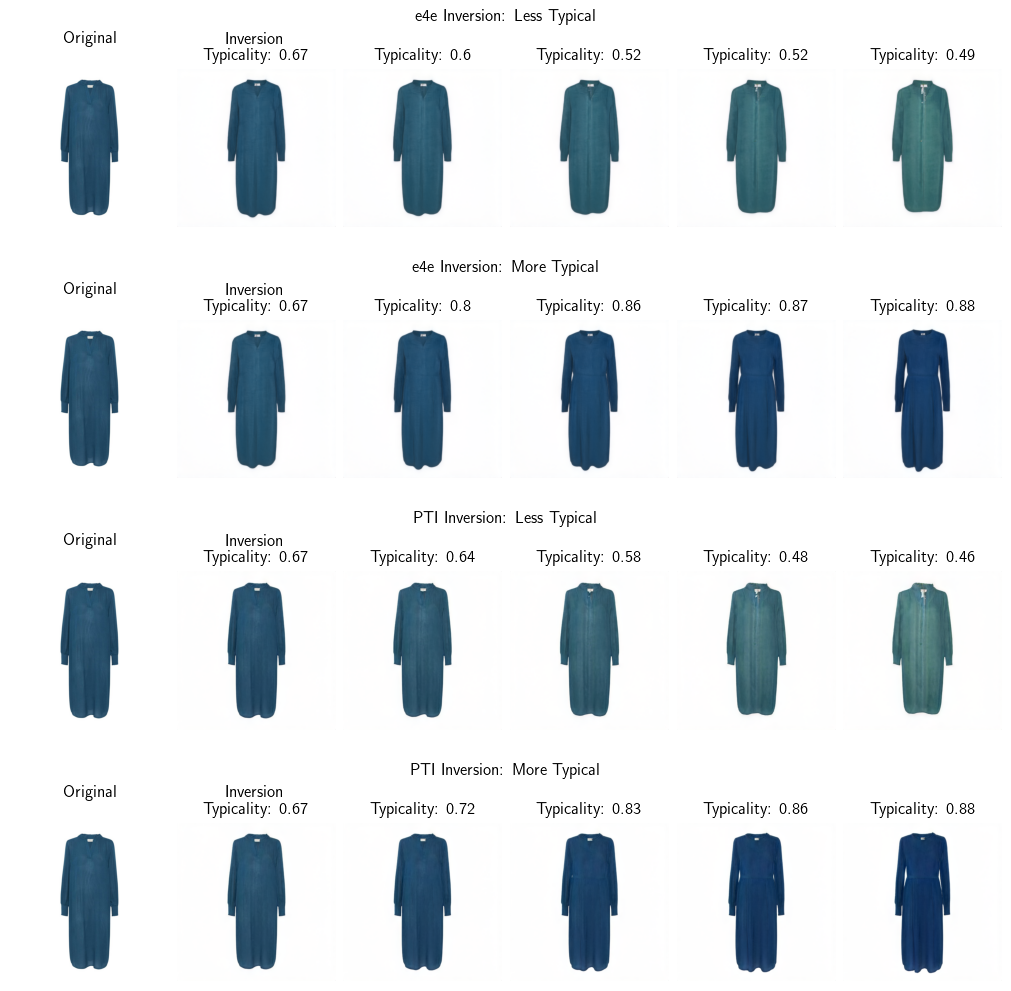
\includegraphics[width=1\linewidth]{Thesis/Results/assets/dino_main_results.png}
    \caption[Typicality Manipulations using DINOv2 Embeddings]{Typicality Manipulations using DINOv2 Embeddings}
    \label{fig:dino_main_results}
\end{figure}

\begin{figure}[!ht]
    \centering
    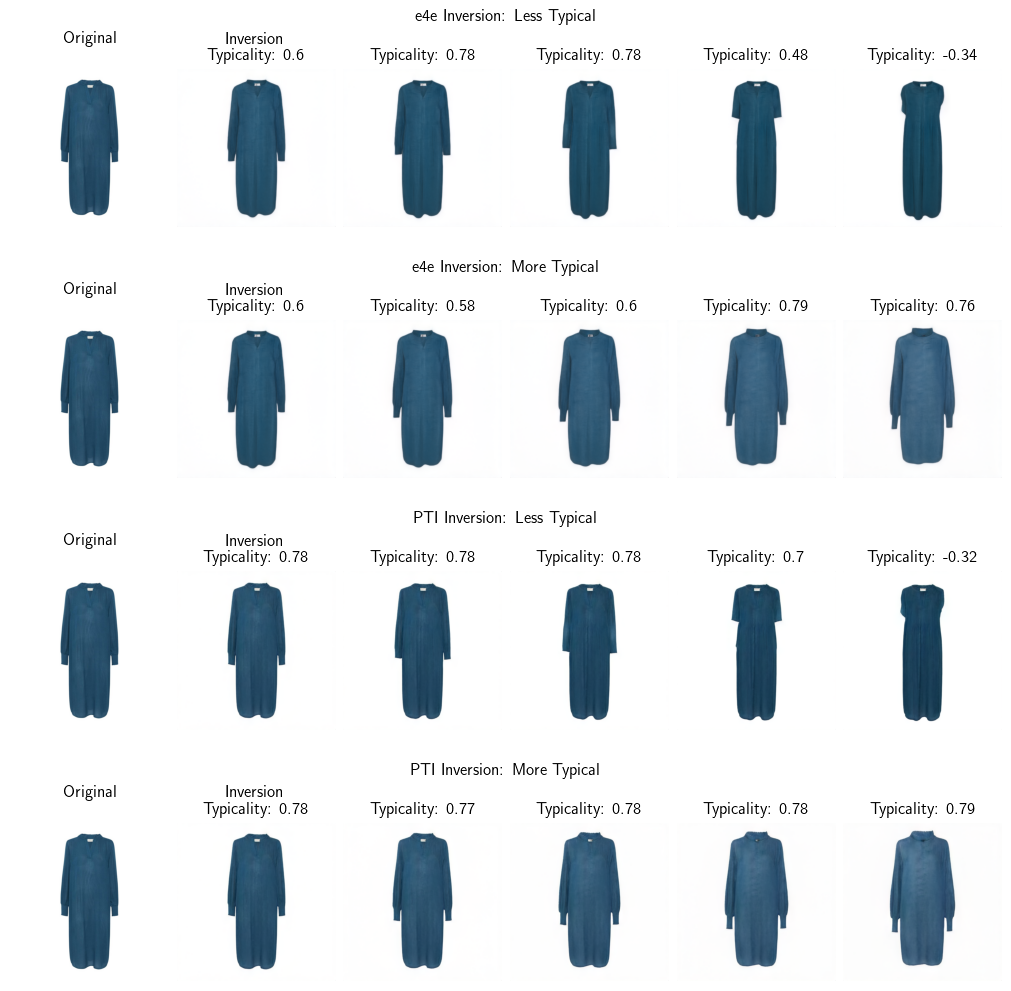
\includegraphics[width=1\linewidth]{Thesis/Results/assets/disentangled_main_results.png}
    \caption[Typicality Manipulations using Disentangled Embeddings]{Typicality Manipulations using Disentangled Embeddings}
    \label{fig:disentangled_main_results}
\end{figure}

For the final typicality manipulation, I compare the two typicality measures against each other, i.e. typicality based on simple DINOv2 embeddings against typicality based on disentangled embeddings. For both embedding types, only e4e and PTI inversions are considered, since those performed well enough in the preliminary experiments. The results of the typicality manipulation based on DINOv2 embeddings and disentangled embeddings for one article (SKU: KA321C13K-K11) are shown in figure \ref{fig:dino_main_results} and \ref{fig:disentangled_main_results} respectively. These figures depict manipulations using incremental InterFaceGAN steps, with each step representing a five-unit shift along the unit-normal vector of the separation boundary - positive for increasing typicality and negative for decreasing it. More examples of manipulations using DINOv2 embeddings can be found in figures \ref{fig:dino_less} and \ref{fig:dino_more} for decreased and increased typicality respectively. Analogously, figure \ref{fig:disentangled_less} and \ref{fig:disentangled_more} show further results for disentangled embeddings. \\
\textbf{Manipulation smoothness} comparisons of typicality scores reveal that typicality scores based on disentangled embeddings change less smoothly, as seen in the abrupt jumps in scores between manipulation steps. This contrasts with the much smoother transitions observed in DINOv2-based manipulations, and this pattern holds for both e4e and PTI inversions. Additionally, the distribution of typicality scores for all reconstructions in the dataset, shown in figure \ref{fig:typicality_score_distribution}, indicates that scores from disentangled embeddings are more dispersed and less smoothly distributed than those based on DINOv2. This likely accounts for the less smooth typicality score manipulations observed with disentangled embeddings. \\
The \textbf{physical attribute changes} that the manipulation does to the dresses, significantly differs between the two typicality measures. For DINOv2-based typicality scores, the changes in the dresses are mostly subtle, primarily involving fine-grained adjustments in shape or color. This observation is in line with the most and least typical dresses based on this embedding type, as shown in figure \ref{fig:examples_dino_typicality} where the most typical dresses are fitted around the waist. Consequently, the manipulation technique tends to make a dress more fitted around the waist when increasing typicality and less fitted when decreasing it. In contrast, typicality manipulation based on disentangled embeddings leads to less subtle changes, significantly altering physical attributes such as sleeve lengths. As shown in figure \ref{fig:disentangled_main_results} and especially in figure \ref{fig:disentangled_more}, to make a dress more typical, long sleeves are added to sleeveless dresses, while sleeves are shortened or transformed into spaghetti straps to make a dress less typical (figure \ref{fig:disentangled_less}). This observation is consistent with the most and least typical dresses shown in figure \ref{fig:examples_disentangled_typicality}, where the most typical dresses have all long sleeves. Those results again hold for both e4e and PTI inversions equally.\\
\begin{figure}[!ht]
    \centering
    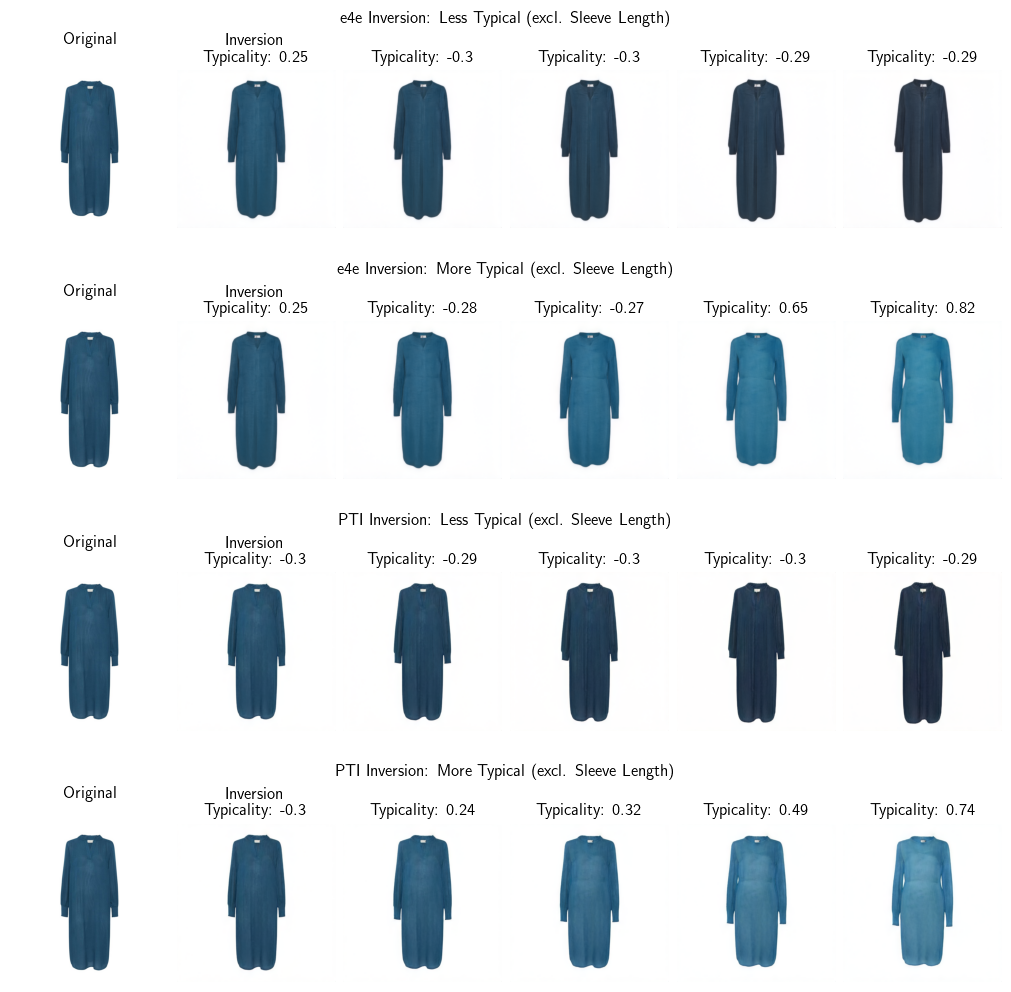
\includegraphics[width=1\linewidth]{Thesis/Results/assets/disentangled_excl_sleeve_main_result.png}
    \caption[Typicality Manipulations using Disentangled Embeddings excl. sleeve length]{Typicality Manipulations using Disentangled Embeddings excl. Sleeve Length}
    \label{fig:disentangled_excl_sleeve_main_result}
\end{figure}
\textbf{Conditional manipulation} using physical attributes like sleeve length can offer valuable insights into the manipulation behavior. By excluding the sleeve length sub-embedding from the disentangled embeddings, the typicality calculation ignores this attribute. During manipulation, this conditioning ensures that the sleeve length cannot change when altering typicality. The results of this conditional typicality manipulation are shown in \ref{fig:disentangled_excl_sleeve_main_result} and \ref{fig:disentangled_ex_sleeve_more}. Since here the typicality manipulation does not entail changes in the sleeve lengths, conditioning works successfully. Additionally, without access to the sleeve length attribute, the manipulations become subtler, focusing instead on adjusting the fit around the waist and making slight color changes. These modifications are consistent with the most and least typical images based on disentangled embeddings excluding sleeve length, as seen in figure \ref{fig:examples_disentangled_ex_sleevel_length}. When applying the same conditioning approach using color as the attribute, the model again relies on sleeve length, as in the unconditional case (see figure \ref{fig:disentangled_ex_color_more}). These experiments reveal that the manipulation model based on disentangled embeddings always opts for the quickest path to typicality, which typically involves altering sleeve lengths. If this attribute is restricted, the model shifts to the next most effective path, adjusting shape and color. This demonstrates that typicality in disentangled embeddings is multi-dimensional, with each dimension contributing to the manipulation of a dress's typicality. Without conditioning, the model naturally selects the most dominant attribute for manipulation. To determine whether this behavior is unique to disentangled typicality manipulation, conditional manipulation was also tested with DINOv2-based typicality scores. Since the unconditional manipulations in this case primarily relied on shape and color, conditioning on color was examined. Conditioning on shape was not feasible due to a mismatch between the dataset's shape attribute and the actual changes seen in manipulation. Results of the color-conditioned typicality manipulation of DINOv2-based embeddings can be found in figure \ref{fig:dino_cond_color_more}. Here it becomes clear, that the conditioning approach in InterFaceGAN does not effectively constrain the color attribute, as the model continues to alter the color of dresses. Furthermore, no significant difference is observed compared to the unconditional manipulation. This indicates that DINOv2-based typicality is driven by a single dimension of typicality, in contrast to the richer, multi-dimensional nature of disentangled embeddings. It is also important to note that the two conditioning methods are not directly methodologically comparable, with one being a post-processing approach, while the other is a complete re-calculation of the typicality measures conditioned on an attribute. For the simple DINOv2 embeddings, conditioning entails ex-post transformation through a projection of the typicality boundary with the respective boundary of the physical attribute, as described in section \ref{sec:interfacegan}. For the typicality measure based on disentangled embeddings, conditional manipulation works by calculating a separate typicality measure and InterFaceGAN boundary based on a concatenation of all sub-embeddings excluding the respective sub-embedding for the attribute at hand.


\textbf{Differences between e4e and PTI inversions} with respect to the manipulation performance can be observed in all result figures. Specifically, generations using PTI inversions tend to deteriorate in quality as the manipulation distance increases. Although PTI reconstructions are generally better than e4e inversions, the last few manipulation steps, i.e. 15-20 unit-normal vector steps away from the reconstruction, often show a decline in image quality. This is likely because the fine-tuned generator in PTI is optimized for the area around the initial reconstruction. When manipulations are performed in the latent space, the resulting latent codes might fall outside the region for which the fine-tuned generator was optimized. This phenomenon is not equally present in all examples. Easy-to-invert dresses require fewer changes in the generator weights, thus being closer to the original generator that can operate well on the whole latent space. For those dresses, quality deterioration is not an issue. However, for dresses with complex patterns or shapes, image quality tends to decline as the distance from the initial reconstruction increases. This observation holds true for both typicality measures.

\FloatBarrier


